\chapter{Die neue Anwendung \emph{CleverMail}}
\label{cha:clevermail}
In diesem Kapitel wird das Konzept von \emph{CleverMail} erörtert, wobei \emph{CleverMail} die bestehende Anwendung \emph{CCMail} ablösen wird. Im Gegensatz zu \emph{CCMail} wird aus der Sicht von \emph{CleverMail} das Gesamtsystem aus mehreren Anwendungen bestehen, die in der Lage sein müssen, \emph{E-Mails} zu versenden. Bis heute ist \emph{clevercure} angewachsen und es wurden neue Anwendungen hinzugefügt, die Aufgrund der Architektur von \emph{CCMail} nicht in \emph{CCMail} eingebunden werden konnten bzw. man sich dazu entschieden hat, die Einbindung zu unterlassen.
\newline
\newline
Folgende Auflistung zeigt alle Anwendungen, die \emph{CleverMail} nutzen werden:
\begin{enumerate}
	\item\emph{CleverWeb}, ist die Web-Anwendung für den webbasierten Zugriff auf \emph{clevercure}.
	\item\emph{CleverInterface}, ist die Schnittstellen Anwendung für den Datenimport und Datenexport.
	\item\emph{CleverSupport (neu)}, ist die Web-Anwendung für die \emph{Support}-Abteilung.
	\item\emph{CleverDocument (neu)}, ist das Dokumentenmanagementsystem, welches von allen Anwendungen genutzt wird.
\end{enumerate}
\ \newline
Im Gegensatz zu \emph{CCMail} soll \emph{CleverMail} nicht als Konsolen-Anwendung, sondern als eigenständige Komponente implementiert werden, die in einem Applikationsserver, der die JEE7-Plattform-Spezifikation unterstützt, betrieben werden kann.
\newpage
Mit der Nutzung der JEE7-Plattform-Spezifikation stehen \emph{CleverMail} eine Vielzahl von Möglichkeiten und Bibliotheken zur Verfügung wie z.B.: 
\begin{enumerate}
	\item\emph{JAX-RS 2.0} (Java Api for RESTful Web Services 2.0),
	\item\emph{EJB 3.1} (Enterprise Java Bean. Standard Komponenten für die Entwicklung in Java Enterprise Containern), 
	\item\emph{JPA 2.1} (Java Persistence Api. Java Schnittstelle für Datenbankzugriffe), 
	\item\emph{JTA 1.2} (Java Transaction Api. Java Schnittstelle für den Support von verteilten Transaktionen), 
	\item\emph{JSF 2.2} (Java Server Faces. Java Spezifikation für die Entwicklung von Webanwendungen) und 
	\item\emph{CDI 1.2} (Context and Dependency Injection. Java Spezifikation eines IOC-Containers (Inversion of control container)).
\end{enumerate}
\ \newline
Diese Bibliotheken werden es erlauben, die Anwendung \emph{CleverMail} so flexibel wie möglich zu gestalten, bringen aber auch ein erhöhtes Maß an Komplexität beim Design mit sich. 
\newline
\newline
\cite[5-6]{patternsOfEnterprise} führt einige Beispiel für \emph{Enterprise}-Anwendungen an, um zu illustrieren, dass jede dieser Anwendungen seine eigenen Probleme und Komplexität mit sich bringt. Daher ist beim Erstellen einer Architektur einer \emph{Enterprise}-Anwendung die konkrete Nutzung zu berücksichtigen. Der Prozess der Konzeption einer Architektur ist ein kreativer Prozess, wobei Konzepte, \emph{Best-Practise} usw. als Unterstützung anzusehen sind und es keinen echten Leitfaden gibt, an dem man sich orientieren kann. Die Architektur wird stark von der konkreten Anwendung beeinflusst. Daher kann sich die Architektur je nach Anwendung stark unterschieden.

\section{Systemaufbau}
Im Gegensatz zum Systemaufbau aus der Sicht von \emph{CCMail}, beschrieben in Abbildung \ref{sec:ccmail-systemaufbau}, soll die Datenbank nicht mehr als Schnittstelle zwischen den Anwendungen und \emph{CleverMail} fungieren. Die Datenbank soll weiterhin ein zentraler Bestandteil von \emph{CleverMail} sein, jedoch soll die Datenbank von den Anwendungen abstrahiert werden. Damit erreicht man, dass die Anwendungen eine einheitliche Schnittstelle nutzen und nicht ihrerseits eigene Schnittstellen zur Datenbank implementieren und warten müssen.
\newpage
\begin{figure}[h]
\centering
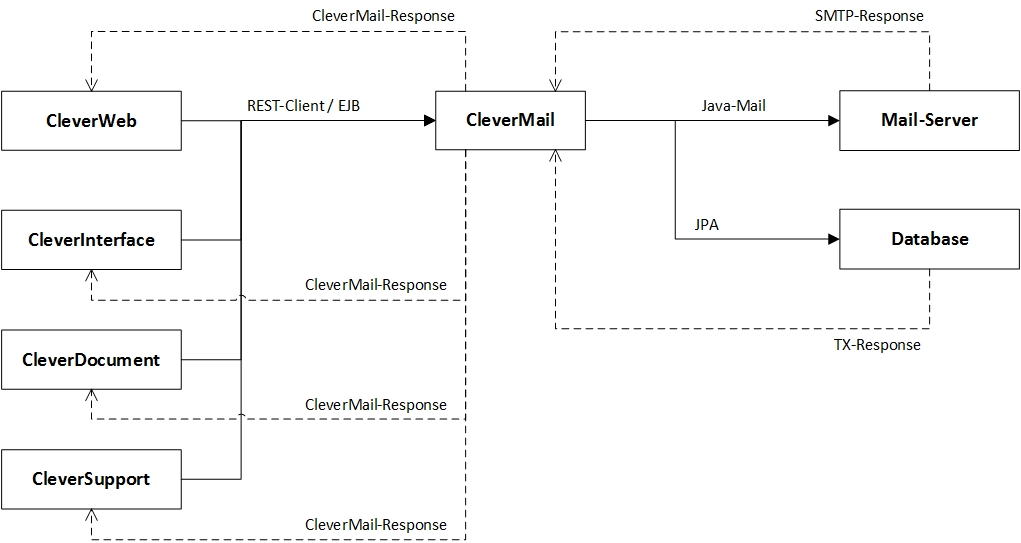
\includegraphics[scale=0.58]{clevermail_systemaufbau.jpg} %{CS0031}
\caption{Systemaufbau und Integration von \emph{CleverMail}}
\label{fig:clevermail-system-und-integration}
\end{figure}
\ \newline
Wie in der Abbildung \ref{fig:clevermail-system-und-integration} illustriert, wird als zentrale Schnittstelle \emph{CleverMail} bzw. dessen implementierte \emph{Client-API} fungieren, wobei diese \emph{Client-API} sich wie folgt ausprägen könnte:
\begin{enumerate}
	\item\emph{REST-Client}, eine REST-Schnittstelle zu einem \emph{REST-Webservice}, über den die zur Verfügung gestellten Funktionalitäten genutzt werden können.
	\item\emph{EJB}, ein EJB (Enterprise Java Bean), welches die zur Verfügung gestellten Funktionalitäten bereitstellt.
\end{enumerate}
\ \newline
\emph{CleverMail} ist für das Persistieren und das Versenden der \emph{E-Mail} verantwortlich und trennt diese Aufgaben vollständig von den Anwendungen. So kann die Wartung an einer Stelle erfolgen und muss nicht über alle Anwendungen hinweg erfolgen. In den Anwendungen würden nur noch Änderungen an den Schnittstellen von \emph{CleverMail} Eingriffe erfordern.
\newline
\newline
Dieser Ansatz würde das Problem der eigens implementierten Datenbankzugriffe beschrieben in Absatz \ref{sec:ccmail-systemaufbau} lösen. Ein Problem könnten hier etwaige technologische Unterschiede darstellen, wie z.B.:
\begin{enumerate}
	\item \emph{REST} nicht verfügbar,
	\item \emph{EJB} nicht verfügbar oder
	\item eine falsche Java-Version.
\end{enumerate}
\ \newline
Obwohl diese Probleme auftreten können, kann zumindest gewährleistet werden, dass alle Anwendungen dieselbe Schnittstelle und dasselbe Domänenmodell verwenden, selbst wenn eigene Implementierungen erforderlich sind. Diese Implementierungen würden Softwarekomponenten von \emph{CleverMail} darstellen und dürfen nicht von den Anwendungen selbst bereitgestellt werden.
Diese technologischen Unterschiede könnten wie folgt gelöst werden:
\begin{enumerate}
	\item\emph{REST}, Integration von JAX-RS 2.0. 
	\item\emph{EJB}, Integration eines EJB-Containers, zur Verfügung stellen eines \emph{Wrappers} oder eine eigene Implementierung des spezifizierten Schnittstellen.
\end{enumerate}

\subsection{1. Möglichkeit \emph{(REST-Client)}}
Eine \emph{REST-Client-API}, welche sich mit JAX-RS 2.0 einfach realisieren lässt, würde ein hohes Maß an Abstraktion bieten, nur eine geringe Kopplung aufweisen und wenig Abhängigkeiten in den Anwendungen erfordern, die den \emph{REST-Client} verwenden. Dem steht aber gegenüber, dass \emph{REST-Services} zustandslos sind und sich daher nicht in Datenbank-Transaktionen einbinden lassen. Dies könnte aber erforderlich sein, wenn eine \emph{E-Mail} nur dann angelegt und versendet werden darf, wenn die Transaktion erfolgreich abgeschlossen wurde (z.B. beim Anlegen einer Bestellung). Für einen \emph{REST-Service} startet der Lebenszyklus mit dessen Aufruf und endet mit dem Übermitteln der Antwort oder wenn die Aktion abgeschlossen wurde (asynchron).
\newline
\newline
Für diese Problem gibt es eine Lösung in Form eines Konzeptes mit der Bezeichnung Try-Confirm-Cancel (TCC).
\begin{figure}[h]
\centering
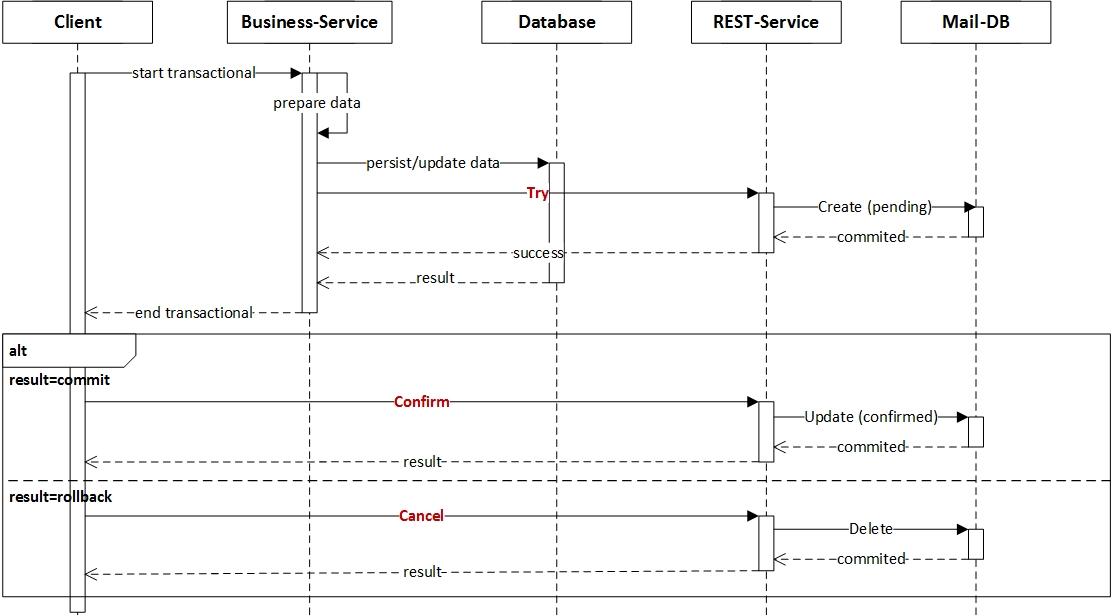
\includegraphics[scale=0.53]{try_confirm_cancel.jpg} %{CS0031}
\caption{Beispiel einer Transaktion mit TCC}
\label{fig:clevermail-rest-tcc}
\end{figure}
\ \newline
Mit dem Konzept \emph{TCC} hält der \emph{REST-Service} die \emph{E-Mail} persistent, markiert die \emph{E-Mail} aber als \emph{unconfirmed}, damit diese \emph{E-Mail} in keiner Verarbeitungslogik miteinbezogen wird. Nach dem erfolgreichen Abschluss der Transaktion auf der \emph{Client}-Seite bestätigt der \emph{Client} den durch den \emph{REST-Service} persistent gehaltenen Zustand, und im Falle eines Fehlers erklärt der \emph{Client} den Zustand für ungültig. Dies erfordert zwei Aufrufe zu REST-Services. Ebenfalls sollte die Transaktion über einen Transaktionskoordinator auf der REST-Seite kontrolliert werden, was wiederum einen Mehraufwand bedeutet. Dieser Transaktionskoordinator wäre dafür verantwortlich, die REST-Services, die Teil einer logischen Transaktionen sind, zu managen. 
\newline
\newline
Mit \emph{TCC} besteht auch die Gefahr das eine \emph{Heuristic-Exception} auftritt. Eine \emph{Heuristic-Exception} tritt auf wenn ein Teilnehmer der Transaktion eine \emph{Heuristic-Decision} (eigenmächtige Entscheidung) trifft und dadurch Dateninkonsistenzen auf der Datenbank entstehen. Dies ist ein Problem, dass vor allem in verteilten System auftreten kann.
\newline
\newline
Diese Probleme bedeuten aber nicht, dass \emph{REST-Services} nicht in Frage kommen. Lediglich für transaktionale Operationen scheinen sie ungeeignet bzw. der Aufwand, der betrieben werden muss, zu hoch. Ein weiteres Problem kann die Erreichbarkeit des \emph{REST-Service} sein. Sollte dieser einmal ausfallen, oder im Falle einer Neuinstallation nicht erreichbar sein, so müsste man eine Rückversicherung haben und die zu erstellenden \emph{E-Mails} anderweitig zwischenspeichern, wie z.B. in Form einer Textdatei, welche die Daten in Form von JSON (Javascript-Objekt-Notation) enthält.
\newline
\newline
Der Artikel von \cite{atomikosTcc} beschreibt den Prozess von \emph{TCC} mit mehreren involvierten REST-Services gut und detailliert.

\subsection{2. Möglichkeit \emph{(EJB)}}
Sollte eine Anwendung \emph{CleverMail} via dessen zur Verfügung gestellten \emph{EJBs} verwenden, so würde eine starke Kopplung und starke Abhängigkeiten entstehen, da mehr Ressourcen benötigt werden. Ebenso könnte im Gegensatz zu einem \emph{REST-Client} keine eigene Datenbank genutzt werden, da ein Zweiphasen-\emph{Commit} erfolgen müsste. Natürlich würde die Möglichkeit von mehreren verwendeten Datenbanken bestehen, aber man wäre der Gefahr von \emph{Heursitc-Exceptions} ausgesetzt.
\newpage
\begin{figure}[h]
\centering
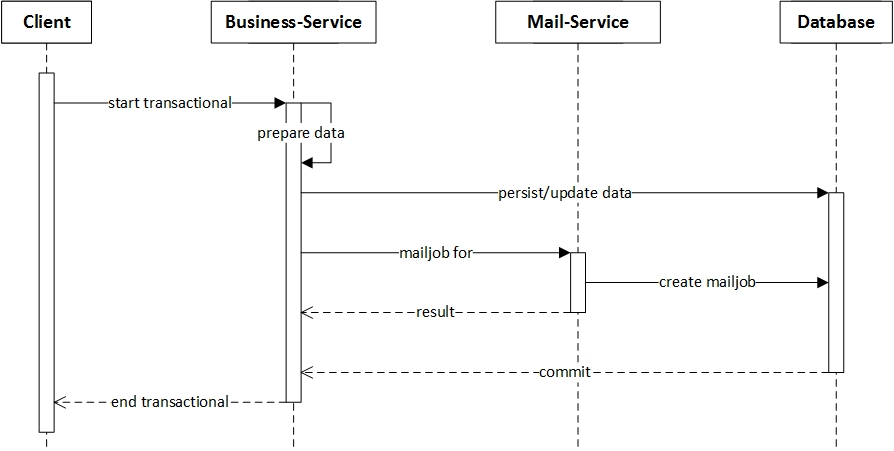
\includegraphics[scale=0.65]{clevermail-ejb-transaktion.jpg} %{CS0031}
\caption{Beispiel einer Datenbanktransaktion mit \emph{EJB}}
\label{fig:clevermail-rest-tcc}
\end{figure}
Wie in Abbildung \ref{fig:clevermail-rest-tcc} illustriert erfolgt das Anlegen einer \emph{E-Mail} in derselben Transaktion und würde daher auch im Falle eines \emph{Rollbacks} entfernt werden. Dies ist sicher die einfachste Art und Weise, um \emph{E-Mails} anzulegen, da hier keine besonderen Mechanismen implementiert werden müssen um die Datenkonsistenz zu gewährleisten. Mit diesem Ansatz wäre die \emph{E-Mail} Teil einer wohldefinierten Transaktion.
\newline
\newline
Wie im Kapitel \ref{cha:clevermail} angemerkt, können technologische Probleme auftreten, wenn z.B. die Laufzeitumgebung einer Anwendung \emph{EJB} und \emph{JTA} nicht zur Verfügung stellt. In so einem Fall müsste man eigene Implementierungen zur Verfügung stellen, die Teil von \emph{CleverMail} sein müssen.
\newline
\newline
Dieser transaktionale Ansatz unterschiedet sich nicht von dem in \emph{CCMail} bereits implementierten, jedoch müssen die von \emph{CleverMail} zur Verfügung gestellten Implementierungen verwendet werden. Diese Implementierungen müssen auch im Backend der \emph{REST-Services} von \emph{CleverMail} verwendet werden, da auch hier die Persistenz der \emph{E-Mails} gewährleistet werden muss.
 
\section{\emph{E-Mail}-Prozesse}
\label{sec:clevermail-prozesse}
Dieser Abschnitt behandelt die Prozessspezifikationen von \emph{CleverMail}. Es wird das Augenmerk auf den Mailversand gelegt. Grundlegend wird sich der \emph{E-Mail}-Versand dadurch unterscheiden, dass mehrere Ebenen involviert sind, bevor eine \emph{E-Mail} bereit zum Versand ist. 
\newline
\newline
Vom grundlegenden Konzept wird sich gegenüber \emph{CCMail} nicht viel ändern. Es soll immer noch \emph{E-Mail}-Typen geben, die aber jetzt nicht nur intern konfigurierbar sein sollen,  sondern ebenfalls durch die KundInnen selbst konfiguriert und gesteuert werden können. Es sollen folgende Konfigurationsmöglichkeiten zur Verfügung stehen.
\begin{enumerate}
	\item Definition von Zeitplänen.
	\item Definition eigener \emph{E-Mail}-Vorlagen.
	\item Konfiguration der Steuerbarkeit von \emph{E-Mail}-Typen durch LieferantInnen (darf aktivieren/de-aktivieren).
	\item Definition eines Haftungsausschluss. 
	\item Definition von Standard-Datei-Anhängen.
	\item Steuerbarkeit von \emph{E-Mail}-Typen für spezifischen LieferantInnen.
	\item Konzernübergreifende Konfiguration.
	\item Definition eigener \emph{E-Mail}-Typen.
	\item Konfiguration der Historie der \emph{E-Mail}-Nachrichten.
\end{enumerate}
\ \newline
Zur Zeit stehen diese Möglichkeiten, wenn vorhanden, nur intern zur Verfügung. Die KundInnen haben lediglich die Möglichkeit, einzelne \emph{E-Mail}-Typen zu aktivieren oder zu de-aktivieren. Diese \emph{E-Mail}-Typen können aber mehrere \emph{E-Mails} halten. Das grundlegende Ziel ist, dass die KundInnen mehr Kontrolle und Konfigurationsmöglichkeiten über die zur Verfügung gestellten \emph{E-Mail}-Typen erhalten. Es wird hier aber auch solche \emph{E-Mail}-Typen geben, bei denen diese Konfigurationsmöglichkeiten eingeschränkt werden. Trotz etwaiger Einschränkungen, sollen die KundInnen in der Lage sein, den \emph{E-Mail}-Verkehr ihrer \emph{E-Mails} besser zu steuern.

\newpage
\subsection{\emph{E-Mail}-Versand}
Folgende Abbildung \ref{fig:clevermail-email-versand} illustriert ein Beispiel eines \emph{E-Mail}-Versands, wobei ein \emph{Client} über eine \emph{REST-Service}-Schnittstelle den Versand von \emph{E-Mails} eines Typs anstößt. Dabei wird der vollständige Prozess eines \emph{E-Mail}-Versands, wie angedacht, dargestellt.
\begin{figure}[H]
\centering
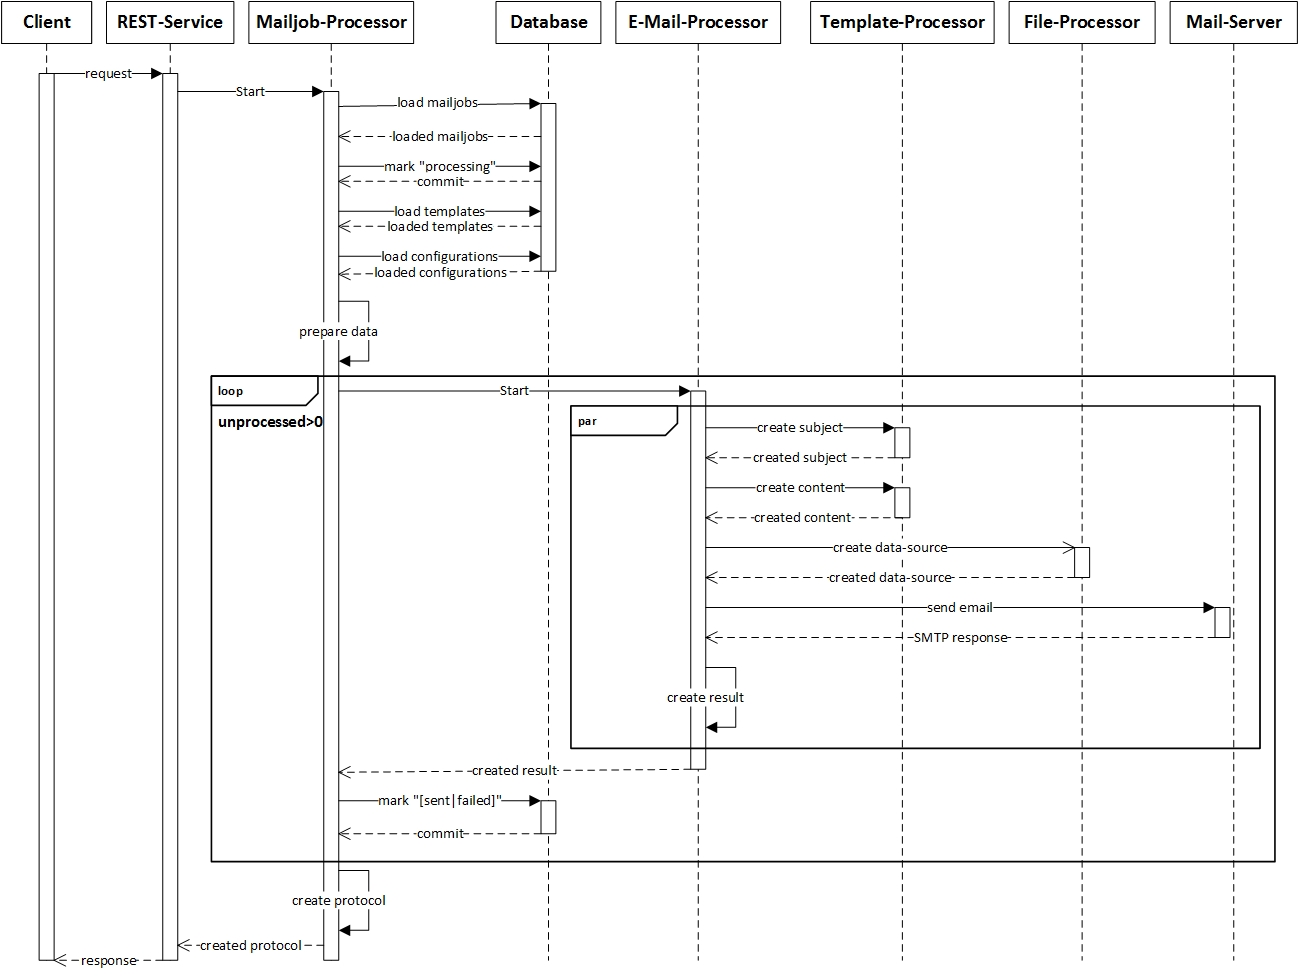
\includegraphics[angle=90, scale=0.6]{clevermail-email-versand.jpg} %{CS0031}
\caption{Prozess des \emph{E-Mail}-Versands}
\label{fig:clevermail-email-versand}
\end{figure}
\ \newline
Der in Abbildung \ref{fig:clevermail-email-versand} dargestellte Prozess wird über eine\emph{REST-Service}-Schnittstelle angestoßen, der in diesem Fall den Prozess synchron abarbeitet und anschließend eine Antwort in Form eines erstellten Reports zurückliefert. Der \emph{REST-Service} ist als optional anzusehen, da dieser Prozess auch anderweitig ausgelöst werden könnte. Nachdem sich dieser Prozess nicht in einer Transaktion eines Client befinden muss, würde sich hier eine REST-Schnittstelle anbieten.
\newline
\newline
Im folgenden sei der Prozess in Unterpunkte unterteilt angeführt und beschrieben:

\subsubsection{1. \emph{MailJob}-Aufbereitung}
Nachdem der Prozess des \emph{E-Mail}-Versands gestartet wurde, müssen die zu verarbeitenden \emph{E-Mails}, repräsentiert durch \emph{MailJobs} aus der Datenbank geladen und mit \emph{Processing} markiert werden. Im Abschnitt \ref{sec:ccmail-email-versand} wurde angemerkt, dass das Problem bestand, dass die in Verarbeitung stehenden \emph{MailJob}-Entitäten nicht als solche markiert wurden und daher eine parallele Verarbeitung durch mehrere Prozesse nicht möglich war. Dieses Problem besteht mit dem Ansatz des Markierens der \emph{MailJob}-Entitäten nicht mehr. Nachdem die \emph{MailJobs} geladen wurden, müssen die zu den \emph{E-Mail}-Typ dazugehörigen \emph{E-Mail}-Vorlagen geladen werden. Es würde sich ein \emph{Cache}-Mechanismus anbieten, da die \emph{E-Mail}-Vorlagen versioniert sind und sich die \emph{E-Mail}-Vorlagen einer Version nicht mehr ändern dürfen. Anschließend werden die kundenspezifischen Konfigurationen geladen. Aus diesen Daten werden Objekte erstellt, die eine \emph{E-Mail} repräsentieren. Diese Modelle werden in weitere Folge dazu verwendet, die tatsächlichen \emph{E-Mails} zu erstellen.

\subsubsection{2. \emph{E-Mail}-Erstellung}
Aus den erstellten Modellen werden die \emph{E-Mails} erstellt. Dabei wird dieser dreiteilige Prozess angewendet:
\begin{enumerate}
	\item\emph{Erstellen des Betreff.} Der Betreff wird aus einer \emph{E-Mail}-Vorlage erstellt und mit Daten befüllt, wenn in der Voralge Parameter definiert wurden.
	\item\emph{Erstellen der Nachricht.} Die Nachricht wird aus einer \emph{E-Mail}-Vorlage erstellt und mit Daten befüllt, wenn in der Vorlage Parameter definiert wurden.
	\item\emph{Erstellen der DataSoruces.} \emph{DataSource}-Objekte halten die Anhänge der \emph{E-Mails}. Die stellen einen \emph{Stream} über die Anhänge der \emph{E-Mail} zur Verfügung.
\end{enumerate}
\ \newline
Die Verarbeitung der \emph{E-Mail}-Vorlagen werden in einer Komponente mit dem Namen \emph{Template-Processor} erfolgen. Nachdem die Werte der verwendeten Vorlagenparameter beim Erstellen eines \emph{MailJobs} in der Datenbank gespeichert wurden, können diese angewandt werden.
\newline
\newline
Die Verarbeitung der Datei Anhänge erfolgt in einer Komponente mit dem Namen \emph{File-Processor}, welche die verlinkten Dateianhänge in Form von \emph{DataSource}-Objekten dem \emph{E-Mail}-Objekt zur Verfügung stellt. Beim Versand würde die das \emph{E-Mail}-Objekt den Dateianhang über die verfügbaren \emph{DataSource}-Objekte laden. Dabei werden die Dateien in Form von Links aus dem Dokumentenmanagementsystem \emph{CleverDocument} geladen. Es dürfen keine Dateien in Form von Base64-Zeichenketten in der Datenbank gespeichert werden, damit die Datenbank nicht mit unnötigen Daten belastet wird. Es könnten hierbei verschiedene \emph{DataSource}-Implementierungen zur Verfügung gestellt werden, welche die Dateien aus verschiedenen Quellen über verschiedene Protokolle laden können (z.B. REST, SOAP oder HTTP).

\subsubsection{3. \emph{E-Mail}-Versand}
Es sollte angedacht werden den \emph{E-Mail}-Versand sowie die Erstellung der \emph{E-Mail}-Objekte asynchron erfolgen zu lassen, da eine sequenzielle Verarbeitung schlecht für die Performance wäre. Nach dem erfolgreichen oder fehlgeschlagenen Versand einer \emph{E-Mail} werden die verfügbaren Daten des \emph{E-Mail}-Versands in Form eines aufbereiteten Resultates zurückgeliefert. Dabei ist vor allem der \emph{SMTP}-Status relevant, der auf jeden Fall gespeichert werden muss. Damit wird sichergestellt, dass die KundInnen nachvollziehen können, wie der Versand einer \emph{E-Mail} abgearbeitet wurde und mit welchen \emph{Error}-Code in einem Fehlerfall eine \emph{E-Mail} nicht zugestellt werden konnte. Ein fehlgeschlagener Versand könnte folgende Ursachen haben:
\begin{enumerate}
	\item Datei kann nicht geladen werden (nicht vorhanden, \emph{timeout},...).
	\item \emph{Mail-Server} des Empfängers nicht erreichbar.
	\item \emph{Mail-Server} nimmt Nachricht nicht an.
\end{enumerate}
\ \newline
Es kann viele Ursachen haben warum eine \emph{E-Mail} nicht zugestellt werden konnte. Vor allem die \emph{Mail-Server} der KundInnen stellen hierbei einen Unsicherheitsfaktor dar, da diese in unterschiedlicher Art und Weise konfiguriert sein könnten. Diese Konfigurationen könnten dazu führen, dass \emph{E-Mails} nicht beim Empfänger ankommen.

\newpage
\subsection{\emph{E-Mail}-Vorlagen und -Parameter}
Einen weiteren wichtigen Aspekt stellen die \emph{E-Mail}-Vorlagen, deren Parameter und die Verwaltung derer dar. Die Bereitstellung von Vorlagenparametern wird den AnwenderInnen die Möglichkeit bieten, auf kontextabhängige Daten in einer \emph{E-Mail}-Vorlage zugreifen zu können. Dadurch wird die Flexibilität erhöht und die AnwenderInnen werden mehr Freiheiten beim Erstellen einer \emph{E-Mail}-Vorlage bekommen. 
\newline
\newline
Die Vorlagenparameter müssen von den EntwicklerInnen innerhalb eines Kontexts zur Verfügung gestellt werden, wobei hier auch ein Entwicklungsaufwand besteht. Die Vorlagenparameter werden innerhalb deren Kontext evaluiert und in die \emph{E-Mail}-Vorlage eingefügt. Dabei können die Daten aus verschiedenen Objekten oder sogar Objektgraphen kommen. Dies bedeutet, dass die Vorlagenparameter über eine spezielle Implementierung ausgelesen werden müssen, die leicht wartbar gehalten werden muss. 
\newline
\newline
Die Vorlagenparameter werden über mehrere Softwarekomponenten hinweg verwendet, die sich in verschiedenen Laufzeitumgebungen befinden dürfen. Daher wird es erforderlich sein, die Vorlagenparameter in einem übergreifenden Modell zu definieren oder über sie von einem Modell in ein anderes Modell über Zuordnungen wie z.B. \emph{Annotations} zu definieren.
\begin{figure}[h]
\centering
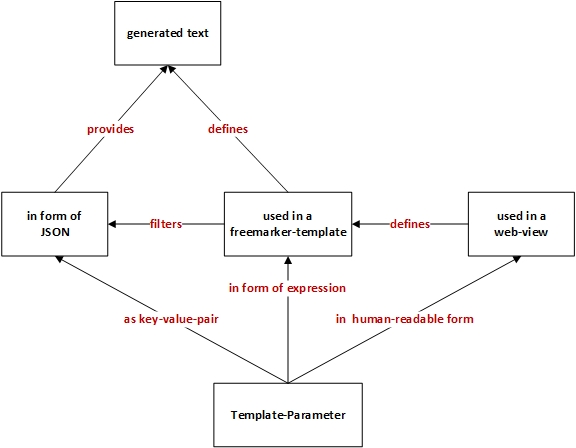
\includegraphics[scale=0.55]{clevermail_template_parameter.jpg}
\caption{Verwendung von Vorlagenparametern}
\label{fig:clevermail-template-parameter}
\end{figure}
\ \newline
Wie in der Abbildung \ref{fig:clevermail-template-parameter} illustriert, werden die Vorlagenparameter in verschiedenen Verwendungskontext und Darstellungen verwendet. Dadurch stellt sich die Frage, wie diese Vorlagenparameter adressiert werden. Man könnte eine Zuordnung in jedem Verwendungskontext erstellen, also jeder Verwendungskontext bekommt sein eigenes Modell. Dadurch würde man zwar lose and die Vorlagenparameter gekoppelt sein , jedoch erhält man auch eine Modell-Klasse je Verwendungskontext, die gewartet werden muss. 

\subsubsection{Verwendungskontext Webseite}
\label{sec:template-parameter-web-view}
Da die Vorlagenparameter in \emph{E-Mail}-Vorlagen verwendet werden, wird es auch eine Webseite geben müssen, über die die AnwenderInnen die Vorlagenparameter in Ihren \emph{E-Mail}-Vorlagen verwenden können. Die Vorlagenparameter müssen für die AnwenderInnen einen Namen bekommen, der auch in mehreren Sprachen zur Verfügung stehen muss. Dadurch werden die Vorlagenparameter auf einen Schlüssel zugeordnet, der wiederum auf einen lokalisierten Spracheintrag zugeordnet ist. Die Zuweisung auf diesen Schlüssel ist erforderlich, aber eine Abstraktion der Vorlagenparameter für die Webseite bzw. deren \emph{Backend} wäre übertrieben.

\subsubsection{Verwendungskontext \emph{Freemarker}-Vorlagen}
\label{sec:template-parameter-freemarker}
Ein weiterer Aspekt ist auch die direkte Verwendung der Vorlagenparameter in der \emph{Freemarker}-Vorlage selbst. Als \emph{Template-Enginge} wird für die Erstellung der \emph{E-Mails} aus den \emph{E-Mail}-Vorlagen \emph{Freemarker} (Frei verfügbare \emph{Template-Engine} in Java für die Erstellung von dynamischen Textdateien) verwendet. Diese Bibliothek ist eine beliebte und gut gewartete Bibliothek, welche alle benötigten Kontrollstrukturen sowie \emph{Freemarker Expressions} zur Verfügung stellt. Diese \emph{Freemarker Expressions} ähneln den \emph{Java EL Expressions} (\emph{Java Expression Language} ist eine Java-Spezifikation für \emph{Expressions}). Die Vorlagenparameter werden in den \emph{Freemarker Expressions} verwendet, die es ermöglichen, eine flache Adressierung sowie auch eine Adressierung über Objektgraphen zu definieren. Auch im Verwendungskontext der \emph{Freemarker Expressions} ist eine Notwendigkeit einer Abstraktion der Vorlagenparametern in Frage zu stellen.

\subsubsection{Verwendungskontext JSON}
\label{sec:template-parameter-json}
Wenn eine \emph{E-Mail} in Form eines \emph{MailJobs} erstellt wird, müssen zum jeweiligen Erstellungszeitpunkt alle Vorlagenparameter evaluiert werden und mit dem \emph{MailJobs} persistent gehalten werden. Nachdem die Anzahl der Vorlagenparameter dynamisch ist und diese Daten lediglich in der Vorlagenverarbeitung verwendet werden, ist es nicht erforderlich eine eigene Datenstruktur in der Datenbank zu definieren. Daher würde sich hier \emph{JSON} anbieten, um diese Daten in die Datenbank zu speichern. Nachdem \emph{JSON} eine Objektbeschreibung mit Zeichenketten darstellt und auch über ein \emph{JSON}-Schema spezifiziert werden kann, sollte man überlegen, ob man nicht \emph{JSON} als Spezifikation für die Vorlagenparameter heranzieht. Diese Spezifikation kann in allen involvierten Komponenten verwendet werden. 

\section{\emph{CleverMail}-Datenbank}
Zusätzlich zur Persistenz der \emph{E-Mails} soll auch die Möglichkeit bestehen, den \emph{E-Mail}-Versand zu konfigurieren. Dies soll einerseits innerhalb des Betriebes möglich sein und andererseits auch für die AnwenderInnen der KundInnen. Dabei sollen folgende Möglichkeiten zur Verfügung stehen:
\begin{enumerate}
	\item Zeitsteuerung des Versands.
	\item Berechtigungen für Modifikationen der \emph{E-Mail}-Vorlagen steuern.
	\item Eigene E\emph{-Mail}-Typen definieren.
	\item Eigene \emph{E-Mail}-Vorlagen definieren.
	\item Zusatzdokumente für \emph{E-Mails} definieren. 
	\item Speicherverwaltung der \emph{E-Mails} steuern.
\end{enumerate}
\ \newline
Um diese Konfigurationen zu verwalten wird ein Speichermedium benötigt, welches auch in der Lage sein muss, die nötigen Relationen abzubilden. Da bietet sich eine relationale Datenbank an. Auch in der alten Anwendung \emph{CCMail} wurde eine relationale Datenbank verwendet und dies soll auch für die neue Anwendung \emph{CleverMail} gelten. Dabei kann das bestehende Datenbankschema von \emph{CCMail} außer Acht gelassen werden und ein vollständig neues Datenbankschema konzipiert werden. 
\newline
\newline
Im Gegensatz zum Datenbankschema von \emph{CCMail}, beschrieben im Abschnitt \ref{sec:ccmail-datanbank}, darf keineswegs auf die referenzielle Integrität zwischen den Tabellen-Relationen verzichtet werden. Dies stellt die größte Fehlentscheidung beim Design des Datenbankschemas von \emph{CCMail} dar. Des weiteren soll so gut wie möglich auf die Unabhängigkeit des Datenbankschema geachtet werden. Damit ist gemeint, dass die Tabellen des Datenbankschemas von \emph{CleverMail} nicht Tabellen der Anwendung \emph{Clevercure} referenzieren dürfen. Dadurch wird sichergestellt, dass das Datenbankschema von \emph{CleverMail} auch ohne \emph{Clevercure} verwendet werden kann. Sollten Referenzen auf Tabellen des Datenbankschemas von \emph{Clevercure} wie Benutzer (\emph{USER}), Kunde (\emph{COMPANY}) eingeführt werden, so kann \emph{CleverMail} nicht außerhalb des Kontextes von \emph{clevercure} existieren und würde immer nur für \emph{Clevercure} zur Verfügung stehen. Das Modul \emph{CleverMail} sollte aber auch als \emph{Standalone}-Anwendung funktionsfähig sein, auch wenn es für die Anwendung \emph{Clevercure} entwickelt werden soll. 
\newline
\newline
Dies begründet sich durch die Anwendungsfälle selbst, die nicht auf eine bestimmte Repräsentation von Inhabern von persistenten \emph{E-Mail}, \emph{E-Mail}-Typen oder Konfigurationen angewiesen sind. Mann muss sich hier die Möglichkeiten für eine zukünftige Anwendung in anderen Anwendungen offen zu halten, anstatt sich den Aufwand einer umfangreichen Umstrukturierung, beim Eintreffen eines solchen Falles, auszusetzen. 
\newline
\newline
Auch wenn der Ansatz der größtmöglichen Abstraktion von \emph{Clevercure} verfolgt werden soll, ist es trotzdem möglich Referenzen auf Tabellen des Datenbankschemas von \emph{Clevercure} herzustellen, solange der Datenzugriff gekapselt und nur einer Stelle gehalten wird. Somit ist gewährleistet, dass eine Umstrukturierung keine unerwünschten Nebeneffekte hat und Änderungen nur an definierten Stellen stattfinden müssen. \cite[66]{refactoreDatabase} beschreiben es wie folgt:
\begin{quote}
\emph{You could implement the SQL logic in a consistent manner, such as having save(), delete(), retrieve(), and find() operations for each business class. Or you could implement data access objects(DAOs), classes that implement the data access logic separately from business classes.}
\end{quote}
Natürlich ist der Ansatz mit \emph{DAOs} vorzuziehen, da hier der Datenzugriff gekapselt an einer Stelle und nicht zerstreut über mehrere \emph{Business}-Klassen implementiert wird.
\newpage
Folgendes \emph{ER}-Diagramm (\emph{Entity Relation}-Diagramm) \ref{fig:clevermail-db-schema} illustriert das Datenbankschema von \emph{CleverMail}. Dieses Datenbankschema stellt eine mögliche Grundstruktur dar und ist nicht als endgültig anzusehen.
\begin{figure}[H]
\centering
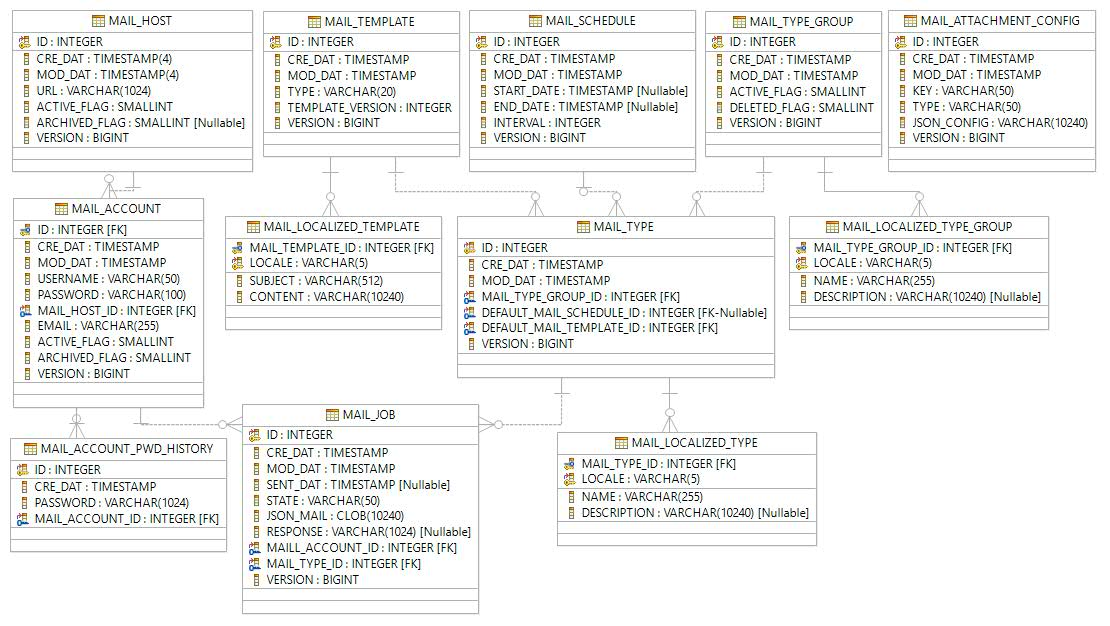
\includegraphics[angle=90, scale=0.44]{clevermail_db_schema.jpg}
\caption{Datenbankschema von \emph{CleverMail}}
\label{fig:clevermail-db-schema}
\end{figure}
Das Datenbankschema aus Abbildung \ref{fig:clevermail-db-schema} enthält keine Referenzen auf das Datenbankschema von \emph{Clevercure}. Die Integration des Datenbankschema von \emph{CleverMail} in das Datenbankschema von \emph{Clevercure} oder visa versa, könnte über N:M-Tabellen abgebildet werden. Mit dieser Art der Tabellenrelation kann auch eine 1:N-Relation abgebildet werden, wobei noch zusätzlich ein \emph{Unique Constraint} auf den Fremdschlüssel der referenzierten Tabelle hinzugefügt werden muss. Mann erhält zwar noch zusätzliche Relationstabellen, die ebenfalls einen zusätzlichen \emph{Join} erfordern, jedoch ist so sichergestellt, dass das Datenbankschema von \emph{CleverMail} unabhängig bleibt.
\newline
\newline
Es ist auch anzumerken, dass das Datenbankschema aus Abbildung \ref{fig:clevermail-db-schema} von \emph{CleverMail} sehr dem Datenbankschema von \emph{CCMail} aus Abschnitt \ref{fig:ccmail-db-schema} ähnelt. Wobei neue Tabellen zu dem Datenbankschema von \emph{CleverMail} hinzugefügt wurden, um die neuen Möglichkeiten wie die Steuerbarkeit des \emph{E-Mail}-Versandes zu ermöglichen. 
\newline
\newline
Die Tabellen, welche die Konfigurationen halten, sollten je nach Anforderung umgesetzt werden, wobei die Möglichkeit Konfigurationen zur Verfügung zu stellen, stets möglich sein soll. Dadurch werden auch die AnwenderInnen der KundInnen nicht unnötig mit nicht benötigten Konfigurationsmöglichkeiten belastet.